\documentclass[12pt]{article}
\usepackage[a4paper, margin=1in]{geometry}
\usepackage{titlesec}
\usepackage{hyperref}
\usepackage{graphicx}
\usepackage{enumitem}
\usepackage{longtable}
\usepackage{array}
\usepackage{ragged2e}
\usepackage{float}
\titleformat{\section}[block]{\large\bfseries}{\thesection.}{0.5em}{}
\titleformat{\subsection}[block]{\normalsize\bfseries}{\thesubsection.}{0.5em}{}


\title{Software Requirements Specification\\\large\textbf{Marito Multilingual Terminology PWA}}
\author{Team Name: Velox}
\date{\today}

\begin{document}

\maketitle
\tableofcontents
\newpage

\section{Introduction}
\subsection{Purpose}
The purpose of this document is to define the software requirements of the Marito system, a multilingual terminology web application developed as part of the COS 301 Capstone project at the University of Pretoria. This document is intended to guide the development team, ensure alignment with client expectations, and serve as a reference for future maintenance, testing, and extension of the platform.

\subsection{Scope}
Marito is a multilingual, progressive web application (PWA) designed to provide users with access to curated statistical terminology in all 11 official South African languages. The system enables users to search and browse glossary terms, submit suggestions, and engage through a gamified contribution model. Marito supports offline functionality, glossary versioning, contributor uploads, and plugin-based feature extensions including AI-enhanced semantic search and analytics. The system is built using a microkernel-microservices architecture for flexibility, modularity, and future extensibility.

\subsection{Intended Audience}
This document is primarily intended for:
\begin{itemize}
    \item \textbf{Developers and engineers} responsible for implementing and maintaining the system.
    \item \textbf{Project stakeholders and academic supervisors} overseeing the design, quality, and alignment of Marito with its educational goals.
    \item \textbf{Testers and QA personnel} who require a clear specification of expected system behavior.
    \item \textbf{Future contributors} who may extend the application or onboard new glossaries and features.
\end{itemize}

\subsection{Document Overview}
The remainder of this document includes detailed user stories, functional and non-functional requirements, architectural and design patterns, service contracts, constraints, and system models. It is structured to follow industry best practices and academic guidelines for software specification documents, ensuring clarity and completeness for all stakeholders.

\subsection{Definitions, Acronyms, and Abbreviations}
\begin{itemize}
    \item \textbf{PWA}: Progressive Web Application
    \item \textbf{CI/CD}: Continuous Integration and Continuous Deployment
\end{itemize}


\section{User Stories}
This section outlines the high-level user goals and core system interactions that informed the functional requirements. Detailed use case specifications and diagrams can be found in the official project repository.

\subsection{User Story \#1: Sync Updates}

\textbf{ID:} US001 (Marito Project) \\
\textbf{Title:} Automatic Synchronization of Downloaded Lexicon Data \\
\textbf{As a:} Marito application user (e.g., language enthusiast, NLP researcher, student) who has downloaded lexicon data for offline use, \\
\textbf{I want:} the application to automatically check for and apply updates to my downloaded lexicon data whenever I am online, \\
\textbf{So that:} I can be confident that I am always working with the most current and accurate version of the linguistic information without needing to manually re-download or check for updates.

\vspace{1em}
\textbf{Acceptance Criteria:}
\begin{enumerate}
    \item \textbf{Automatic Update Check:}
    \begin{itemize}
        \item \textbf{Given} I have previously downloaded lexicon data,
        \item \textbf{And} I open the Marito application with an active internet connection,
        \item \textbf{Then} the application automatically initiates a check for updates to my downloaded data against the central repository in the background.
    \end{itemize}

    \item \textbf{Notification of Available Updates (Recommended):}
    \begin{itemize}
        \item \textbf{Given} updates are available for my downloaded data,
        \item \textbf{Then} the application clearly notifies me that updates are available (e.g., via a subtle in-app notification, a badge on a settings icon).
        \item \textbf{And} the notification provides an option to view details about the updates (e.g., number of terms changed, lexicon version).
    \end{itemize}

    \item \textbf{Update Process:}
    \begin{itemize}
        \item \textbf{Given} updates are available and I have an active internet connection,
        \item \textbf{Then} the application allows me to initiate the download and application of these updates (or this happens automatically, depending on user settings or application design).
        \item \textbf{And} the application provides clear feedback on the progress of the update (e.g., download progress bar, installation status).
        \item \textbf{And} the update process is efficient and minimizes data usage (e.g., by only downloading changes/deltas if possible, rather than the entire dataset, for future enhancements).
    \end{itemize}

    \item \textbf{Successful Update:}
    \begin{itemize}
        \item \textbf{Given} the update process completes successfully,
        \item \textbf{Then} my locally stored lexicon data reflects the latest version from the central repository.
        \item \textbf{And} I receive a confirmation message that the data has been updated.
    \end{itemize}

    \item \textbf{Handling No Updates:}
    \begin{itemize}
        \item \textbf{Given} I am online and no updates are available for my downloaded data,
        \item \textbf{Then} the application does not interrupt my workflow with unnecessary notifications (or provides a subtle indication that data is ``up-to-date'').
    \end{itemize}

    \item \textbf{Offline State Post-Sync:}
    \begin{itemize}
        \item \textbf{Given} my data has been successfully synced,
        \item \textbf{Then} the newly updated data is fully accessible offline.
    \end{itemize}

    \item \textbf{Error Handling - Interrupted Connection:}
    \begin{itemize}
        \item \textbf{Given} an update is in progress and my internet connection is lost,
        \item \textbf{Then} the application gracefully pauses or stops the update process.
        \item \textbf{And} I am notified of the interruption.
        \item \textbf{And} the application attempts to resume the update when the connection is re-established, or allows me to manually retry.
        \item \textbf{And} my previously downloaded (pre-update attempt) data remains intact and usable.
    \end{itemize}

    \item \textbf{Error Handling - Sync Conflict (Advanced Consideration for Future):}
    \begin{itemize}
        \item \textbf{Given} a conflict occurs during synchronization (e.g., if local modifications were possible vs. server changes),
        \item \textbf{Then} the system has a defined strategy for conflict resolution (e.g., prioritizes server version for this project's scope, notifies user if manual intervention were ever needed).
    \end{itemize}

    \item \textbf{User Control (Optional Enhancement):}
    \begin{itemize}
        \item \textbf{Given} I am a user concerned about data usage or update timing,
        \item \textbf{Then} I may have an option in settings to control sync behavior (e.g., sync only on Wi-Fi, schedule syncs, manual sync only).
    \end{itemize}
\end{enumerate}

\vspace{1em}
\textbf{Notes/Assumptions:}
\begin{itemize}
    \item This user story assumes that users primarily download data for offline reading and searching. Contributions and comments are made while online and sent to a central repository (as per Functional Requirement FR4.3).
    \item The complexity of only downloading changes/deltas (Acceptance Criterion 3.4) can be significant. For an initial implementation, syncing entire updated files might be a simpler starting point, with delta updates as a future enhancement.
    \item Conflict resolution (Acceptance Criterion 8) is likely simplified if the local data is treated as a read-only cache that gets overwritten by server updates, which aligns with the current understanding of the Marito project.
\end{itemize}



\subsection{User Story \#2: Download Language Resources for Offline Access}

\textbf{ID:} US002 (Marito Project) \\
\textbf{Title:} Download Select Language Resources for Offline Use \\
\textbf{As a:} Marito application user (e.g., language enthusiast, NLP researcher, student), \\
\textbf{I want:} to be able to select and download specific language resources (like individual lexicons, glossaries, or dictionaries) to my device, \\
\textbf{So that:} I can access and use this information even when I do not have an active internet connection.

\vspace{1em}
\textbf{Acceptance Criteria:}
\begin{enumerate}
    \item \textbf{Discover and Select Resources for Download:}
    \begin{itemize}
        \item \textbf{Given} I am browsing the available language resources within the application (while online),
        \item \textbf{Then} I can clearly identify which resources are available for download.
        \item \textbf{And} I can select one or more language resources to download.
        \item \textbf{And} the application shows the estimated size of the selected resource(s) before initiating the download.
    \end{itemize}

    \item \textbf{Initiate Download:}
    \begin{itemize}
        \item \textbf{Given} I have selected one or more language resources for download,
        \item \textbf{Then} I can initiate the download process with a clear action (e.g., a ``Download'' button).
    \end{itemize}

    \item \textbf{Download Process Feedback:}
    \begin{itemize}
        \item \textbf{Given} a download is in progress,
        \item \textbf{Then} the application provides clear visual feedback on the download status (e.g., progress bar, percentage complete, estimated time remaining).
        \item \textbf{And} I can continue to use other online features of the application while a download is in progress (background download).
        \item \textbf{And} I have the option to pause and resume a download if needed.
        \item \textbf{And} I have the option to cancel an ongoing download.
    \end{itemize}

    \item \textbf{Successful Download and Storage:}
    \begin{itemize}
        \item \textbf{Given} a language resource download completes successfully,
        \item \textbf{Then} the application notifies me that the download is complete.
        \item \textbf{And} the downloaded resource is stored locally on my device in a way that the Marito application can access it offline.
        \item \textbf{And} the application clearly indicates which resources have been successfully downloaded and are available offline.
    \end{itemize}

    \item \textbf{Managing Downloaded Resources:}
    \begin{itemize}
        \item \textbf{Given} I have downloaded language resources,
        \item \textbf{Then} I can view a list of all my downloaded resources within the application.
        \item \textbf{And} I can remove/delete downloaded resources from my device to free up storage space.
        \item \textbf{And} the application shows the amount of local storage space currently used by downloaded Marito resources.
    \end{itemize}

    \item \textbf{Error Handling - Insufficient Storage:}
    \begin{itemize}
        \item \textbf{Given} I attempt to download a resource,
        \item \textbf{And} my device has insufficient storage space,
        \item \textbf{Then} the application informs me of the insufficient storage and the download does not proceed (or pauses until space is freed).
    \end{itemize}

    \item \textbf{Error Handling - Interrupted Connection During Download:}
    \begin{itemize}
        \item \textbf{Given} a download is in progress and my internet connection is lost,
        \item \textbf{Then} the application gracefully pauses the download process.
        \item \textbf{And} I am notified of the interruption.
        \item \textbf{And} the application attempts to resume the download automatically when the connection is re-established, or allows me to manually resume.
    \end{itemize}

    \item \textbf{Error Handling - Download Failure:}
    \begin{itemize}
        \item \textbf{Given} a download fails for reasons other than connection loss or insufficient storage (e.g., server error, corrupted file),
        \item \textbf{Then} the application notifies me of the failure and provides a reason if possible.
        \item \textbf{And} I have the option to retry the download.
    \end{itemize}

    \item \textbf{Accessing Downloaded Resources Offline:}
    \begin{itemize}
        \item \textbf{Given} I have successfully downloaded a language resource,
        \item \textbf{And} I am offline,
        \item \textbf{Then} I can access and use that downloaded resource within the Marito application.
    \end{itemize}
\end{enumerate}

\vspace{1em}
\textbf{Notes/Assumptions:}
\begin{itemize}
    \item The user must be online to browse and initiate downloads.
    \item The application will need appropriate permissions to write to local device storage.
    \item The format of the downloaded data should be optimized for offline use and efficient storage.
    \item This user story focuses on the \textit{download} functionality. A separate user story would cover the specifics of \textit{accessing and using} the data offline (e.g., offline search within downloaded resources).
\end{itemize}


\subsection{User Story \#3: Search Feature}

\textbf{ID:} US003 (Marito Project) \\
\textbf{Title:} Multilingual Term Search \\
\textbf{As a:} Marito application user (e.g., casual user, linguist, or contributor), \\
\textbf{I want:} to search across multiple multilingual glossaries and dictionaries using filters and smart suggestions, \\
\textbf{So that:} I can quickly find definitions, translations, and related entries in my preferred language.

\vspace{1em}
\textbf{Acceptance Criteria:}
\begin{enumerate}
    \item \textbf{Query Input:}
    \begin{itemize}
        \item \textbf{Given} I am on the main search page,
        \item \textbf{When} I enter a query into the search bar,
        \item \textbf{Then} the system searches across all selected data sources and returns matching terms.
    \end{itemize}

    \item \textbf{Filter Options:}
    \begin{itemize}
        \item \textbf{Given} I want to refine my search,
        \item \textbf{Then} I can apply filters like language, part of speech, or glossary type before or after submitting the query.
    \end{itemize}

    \item \textbf{Fuzzy Search (Optional):}
    \begin{itemize}
        \item \textbf{Given} my query has a typo or partial match,
        \item \textbf{Then} the system offers similar results using fuzzy matching.
    \end{itemize}

    \item \textbf{AI-Powered Suggestions (Optional):}
    \begin{itemize}
        \item \textbf{Given} I start typing in the search bar,
        \item \textbf{Then} I see AI-generated autocomplete suggestions based on common terms or semantic matches.
    \end{itemize}

    \item \textbf{Search History:}
    \begin{itemize}
        \item \textbf{Given} I have searched for terms in the past,
        \item \textbf{Then} the system shows my recent queries and allows re-searching them.
    \end{itemize}

    \item \textbf{Sorting and Result Presentation:}
    \begin{itemize}
        \item \textbf{Given} the results are displayed,
        \item \textbf{Then} I can sort them by relevance, alphabetical order, or popularity,
        \item \textbf{And} each result shows the term, language, and a brief definition snippet.
    \end{itemize}
\end{enumerate}

\vspace{1em}
\textbf{Assumptions:}
\begin{itemize}
    \item Offline support will allow previously downloaded glossaries to be searched.
    \item Filters and sort options persist across sessions.
    \item AI and fuzzy search are optional enhancements.
    \item Glossary datasets are already available and preloaded or fetched via sync.
\end{itemize}

\subsection{User Story \#4: Feedback Submissions}
\textbf{ID:} US004 (Marito Project) \\
\textbf{Title:} User Contributions and Feedback \\
\textbf{As a:} logged-in user of the application, \\
\textbf{I want:} to be able to comment on terms and submit feedback or error reports, \\
\textbf{So that:} I can contribute to improving the accuracy and usefulness of the data content.

\vspace{1em}
\textbf{Acceptance Criteria:}
\begin{enumerate}
    \item \textbf{Commenting on Terms:}
    \begin{itemize}
        \item \textbf{Given} I am logged into my account,
        \item \textbf{And} I am viewing a term or entry,
        \item \textbf{Then} I should see a comment section below the entry,
        \item \textbf{And} I should be able to submit my own comment.
    \end{itemize}

    \item \textbf{Submitting Feedback:}
    \begin{itemize}
        \item \textbf{Given} I am logged into my account,
        \item \textbf{And} I am viewing a specific term or entry,
        \item \textbf{And} I choose to provide feedback,
        \item \textbf{Then} I should be presented with a feedback form,
        \item \textbf{And} I should receive a confirmation message after successfully submitting the feedback.
    \end{itemize}

    \item \textbf{Voting on User Contributions:}
    \begin{itemize}
        \item \textbf{Given} I am logged into my account,
        \item \textbf{And} I am viewing a comment or suggestion submitted by another user,
        \item \textbf{Then} I should see upvote and downvote buttons associated with it,
        \item \textbf{And} I should be able to cast one vote per contribution,
        \item \textbf{And} the vote count should update immediately after I vote.
    \end{itemize}

    \item \textbf{Approval Status of Feedback:}
    \begin{itemize}
        \item \textbf{Given} I have submitted feedback for a term,
        \item \textbf{And} the feedback has been approved by a moderator,
        \item \textbf{Then} the approved feedback should be integrated into the application content,
        \item \textbf{And} I should receive a notification confirming the integration.
    \end{itemize}

    \item \textbf{Marking Approved Submissions:}
    \begin{itemize}
        \item \textbf{Given} user feedback or content has been approved and integrated,
        \item \textbf{Then} the associated entry should be visibly marked as a ``User Submission'' to distinguish it from original content.
    \end{itemize}

    \item \textbf{Rewarding User Contributions (Optional Gamification):}
    \begin{itemize}
        \item \textbf{Given} I am logged in and submit a comment, feedback, or report,
        \item \textbf{When} my contribution meets a predefined threshold (e.g., approved, upvoted),
        \item \textbf{Then} I should earn points or badges for that action,
        \item \textbf{And} my contribution stats should be viewable in my profile.
    \end{itemize}
\end{enumerate}

\vspace{1em}
\textbf{Notes/Assumptions:}
\begin{itemize}
    \item Only logged-in users can comment, submit feedback, vote, or receive contribution rewards.
    \item Users must have verified accounts to interact with community features (e.g., comments, voting).
    \item Rate limiting will be implemented to prevent spam submissions.
\end{itemize}

\subsection{User Story \#5: Gamification Feature}

\textbf{ID:} US005 (Marito Project) \\
\textbf{Title:} Contribution-Based Rewards and Progress Tracking \\
\textbf{As a:} frequent Marito contributor (e.g., user who submits suggestions or comments), \\
\textbf{I want:} to earn points, unlock badges, and track my contribution progress, \\
\textbf{So that:} I feel motivated to participate and can see recognition for my efforts.

\vspace{1em}
\textbf{Acceptance Criteria:}
\begin{enumerate}
    \item \textbf{Points for Contribution:}
    \begin{itemize}
        \item \textbf{Given} I submit a suggestion, comment, or report an issue on a term,
        \item \textbf{Then} I earn points based on the type and quality of the contribution.
    \end{itemize}
    
    \item \textbf{Achievement Unlocking:}
    \begin{itemize}
        \item \textbf{Given} I reach a milestone,
        \item \textbf{Then} I unlock a badge or achievement.
    \end{itemize}

    \item \textbf{Progress Dashboard:}
    \begin{itemize}
        \item \textbf{Given} I navigate to my profile,
        \item \textbf{Then} I can view my total points, badges earned, and contribution rank.
    \end{itemize}

    \item \textbf{Real-Time Feedback:}
    \begin{itemize}
        \item \textbf{Given} I perform a gamified action,
        \item \textbf{Then} I receive instant feedback such as a pop-up message.
    \end{itemize}

    \item \textbf{Leveling Up:}
    \begin{itemize}
        \item \textbf{Given} I reach predefined thresholds,
        \item \textbf{Then} my user rank or title updates accordingly.
    \end{itemize}

    \item \textbf{Offline Support:}
    \begin{itemize}
        \item \textbf{Given} I contribute while offline,
        \item \textbf{Then} my contributions and points are synced once I reconnect.
    \end{itemize}
\end{enumerate}

\subsection{User Story \#6: UpVote System}

\textbf{ID:} US006 (Marito Project) \\
\textbf{Title:} Crowdsourced Validation via UpVoting \\
\textbf{As a:} Marito application user (e.g., casual user, linguist, or academic) who wants to contribute to the accuracy and quality of lexicon entries, \\
\textbf{I want:} to upvote (or downvote) suggested changes or comments on terms in the lexicon, \\
\textbf{So that:} the community can collectively validate contributions, and moderators can prioritize high-quality updates for integration into the central repository.

\vspace{1em}
\textbf{Acceptance Criteria:}
\begin{enumerate}
    \item \textbf{Voting Interface:}
    \begin{itemize}
        \item \textbf{Given} I am viewing a term entry with user-submitted comments or suggested changes,
        \item \textbf{Then} I see an option to upvote or downvote each contribution.
        \item \textbf{And} the current vote count is displayed next to each contribution.
    \end{itemize}

    \item \textbf{Vote Submission:}
    \begin{itemize}
        \item \textbf{Given} I am logged in and have not yet voted on a specific contribution,
        \item \textbf{When} I click the upvote/downvote button,
        \item \textbf{Then} my vote is recorded immediately (if online) or queued for sync (if offline).
        \item \textbf{And} the UI reflects my vote and updates the vote count.
    \end{itemize}

    \item \textbf{Prevent Duplicate Voting:}
    \begin{itemize}
        \item \textbf{Given} I have already voted on a contribution,
        \item \textbf{Then} the UI prevents me from voting again (unless I undo my vote).
    \end{itemize}

    \item \textbf{Offline Handling:}
    \begin{itemize}
        \item \textbf{Given} I vote while offline,
        \item \textbf{Then} the vote is stored locally and synced to the central repository when I reconnect.
    \end{itemize}

    \item \textbf{Moderation Visibility (Optional Enhancement):}
    \begin{itemize}
        \item \textbf{Given} I am a moderator,
        \item \textbf{Then} I can filter contributions by vote count to prioritize high-quality submissions.
    \end{itemize}

    \item \textbf{Feedback Transparency:}
    \begin{itemize}
        \item \textbf{Given} a contribution receives significant downvotes,
        \item \textbf{Then} the system may flag it for review (future enhancement).
    \end{itemize}
\end{enumerate}

\vspace{1em}
\textbf{Notes/Assumptions:}
\begin{itemize}
    \item Voting requires user authentication to prevent abuse.
    \item Vote counts are public to encourage transparency.
    \item Offline votes are treated as "pending" until synced.
    \item Future enhancements could include:
    \begin{itemize}
        \item Weighted voting for trusted users (e.g., linguists).
    \end{itemize}
\end{itemize}


\subsection{User Story \#7.1: Word Frequency Trends}

\textbf{ID:} US007.1 (Marito Project) \\
\textbf{Title:} Historical Word Usage Visualization \\
\textbf{As a:} Linguist or language researcher studying lexical evolution, \\
\textbf{I want:} To view historical trends of word usage frequency across different time periods, \\
\textbf{So that:} I can identify patterns in language adoption, obsolescence, or cultural influences.

\vspace{1em}
\textbf{Acceptance Criteria:}
\begin{enumerate}
    \item \textbf{Trend Visualization:}
    \begin{itemize}
        \item \textbf{Given} I select a word or phrase,
        \item \textbf{Then} I see a line chart showing its monthly/quarterly/yearly frequency.
        \item \textbf{And} can toggle between absolute counts and percentage changes.
    \end{itemize}

    \item \textbf{Comparative Analysis:}
    \begin{itemize}
        \item \textbf{Given} I select multiple words,
        \item \textbf{Then} the system overlays their trends with distinct colors.
        \item \textbf{And} provides a legend identifying each word.
    \end{itemize}

    \item \textbf{Contextual Data:}
    \begin{itemize}
        \item \textbf{Given} I hover over a data point,
        \item \textbf{Then} I see exact usage counts and sample sentences.
        \item \textbf{And} can click to view source documents.
    \end{itemize}

    \item \textbf{Export Functionality:}
    \begin{itemize}
        \item \textbf{Given} I want to analyze data externally,
        \item \textbf{Then} I can export charts as PNG or data as CSV/JSON.
    \end{itemize}
\end{enumerate}

\vspace{1em}
\textbf{Notes/Assumptions:}
\begin{itemize}
    \item Data aggregates nightly for performance.
    \item Supports all 12 official South African languages.
    \item Default view shows last 12 months.
    \item Future enhancements could include:
    \begin{itemize}
        \item Regional usage heatmaps.
        \item Sociolinguistic correlation analysis.
    \end{itemize}
\end{itemize}

\subsection{User Story \#7.2: Contribution Analytics}

\textbf{ID:} US007.2 (Marito Project) \\
\textbf{Title:} User Contribution Visualization \\
\textbf{As a:} Regular contributor to the Marito platform, \\
\textbf{I want:} To see a breakdown of my edits and comments across languages, \\
\textbf{So that:} I can track my impact and focus on underrepresented languages.

\vspace{1em}
\textbf{Acceptance Criteria:}
\begin{enumerate}
    \item \textbf{Personal Dashboard:}
    \begin{itemize}
        \item \textbf{Given} I view my profile,
        \item \textbf{Then} I see a pie chart of my contributions by language.
        \item \textbf{And} a timeline of my activity.
    \end{itemize}

    \item \textbf{Progress Metrics:}
    \begin{itemize}
        \item \textbf{Given} I'm an active user,
        \item \textbf{Then} I see my percentile ranking in the community.
        \item \textbf{And} suggested languages needing more contributions.
    \end{itemize}
\end{enumerate}

\vspace{1em}
\textbf{Notes/Assumptions:}
\begin{itemize}
    \item Updates within 5 minutes of contributions.
    \item Includes all contribution types.
    \item Future enhancements could include:
    \begin{itemize}
        \item Team contribution tracking.
        \item Contribution quality scoring.
    \end{itemize}
\end{itemize}

\subsection{User Story \#7.3: Trending Terms}

\textbf{ID:} US007.3 (Marito Project) \\
\textbf{Title:} Real-Time Popularity Tracking \\
\textbf{As a:} Language learner or cultural researcher, \\
\textbf{I want:} To see which words are currently trending in popularity, \\
\textbf{So that:} I can stay current with evolving language usage.

\vspace{1em}
\textbf{Acceptance Criteria:}
\begin{enumerate}
    \item \textbf{Trending Display:}
    \begin{itemize}
        \item \textbf{Given} I visit the homepage,
        \item \textbf{Then} I see a ``Trending Now'' carousel with top terms.
        \item \textbf{And} percentage change indicators.
    \end{itemize}

    \item \textbf{Contextual Information:}
    \begin{itemize}
        \item \textbf{Given} I select a trending word,
        \item \textbf{Then} I see related news/events driving popularity.
        \item \textbf{And} its historical frequency graph.
    \end{itemize}
\end{enumerate}

\vspace{1em}
\textbf{Notes/Assumptions:}
\begin{itemize}
    \item Updates every 4 hours.
    \item Excludes spam/fake trends.
    \item Future enhancements could include:
    \begin{itemize}
        \item User-submitted trend explanations.
        \item Regional trend variations.
    \end{itemize}
\end{itemize}




\vspace{1em}
\textbf{Assumptions:}
\begin{itemize}
    \item Contributions are validated before points are awarded to prevent abuse.
    \item Gamification rewards are symbolic, not monetary.
    \item This feature is designed to encourage consistent, high-quality engagement.
\end{itemize}


\subsection{User Story \#8: Responsive Design}
\textbf{ID:} US008 (Marito Project) \\
\textbf{Title:} Responsive Layout for Mobile and Desktop Devices \\
\textbf{As a:} user who may need to access the Marito application while on the go, \\
\textbf{I want:} the user interface to adapt and remain fully functional on mobile phones, tablets, and desktops, \\
\textbf{So that:} I can quickly and seamlessly use the application in any situation, regardless of the device I'm using.

\vspace{1em}
\textbf{Acceptance Criteria:}
\begin{enumerate}
    \item \textbf{Mobile Adaptability:}
    \begin{itemize}
        \item \textbf{Given} I am using the Marito application,
        \item \textbf{And} I am on a mobile device,
        \item \textbf{Then} the layout should automatically adjust to fit the screen without horizontal scrolling.
    \end{itemize}

    \item \textbf{Touch-Friendly UI:}
    \begin{itemize}
        \item \textbf{Given} I am interacting with the app on a touchscreen device,
        \item \textbf{And} I tap on any button or link,
        \item \textbf{Then} the tapped element should be responsive to touch and have a minimum tap area of 48px × 48px.
    \end{itemize}

    \item \textbf{Touchscreen Swiping and Scrolling Support:}
    \begin{itemize}
        \item \textbf{Given} I am using the Marito app on a touchscreen device,
        \item \textbf{And} I am viewing content that extends beyond the initial screen (e.g., a list or feed),
        \item \textbf{Then} I should be able to scroll vertically or horizontally (depending on the content) using swipe gestures,
        \item \textbf{And} the scrolling should be smooth and responsive.
    \end{itemize}

    \item \textbf{Adaptive Mobile Navigation Elements:}
    \begin{itemize}
        \item \textbf{Given} I am using the Marito app on a mobile device,
        \item \textbf{Then} the navigation should adapt to a mobile-friendly layout, such as displaying a hamburger menu instead of a full-width navigation bar.
    \end{itemize}

    \item \textbf{Device Orientation Handling:}
    \begin{itemize}
        \item \textbf{Given} I am using the app on a mobile device,
        \item \textbf{And} I switch between portrait and landscape mode,
        \item \textbf{Then} the UI layout should follow without breaking or cutting off content.
    \end{itemize}

    \item \textbf{Mobile Hardware and OS Compatibility:}
    \begin{itemize}
        \item \textbf{Given} I am using the Marito app on a mobile device running a supported OS (e.g., Android 10+, iOS 13+),
        \item \textbf{And} the device has at least 2 GB of RAM and a modern mobile browser (e.g., Chrome),
        \item \textbf{Then} all core features should work smoothly without crashes or performance lags.
    \end{itemize}

    \item \textbf{Error Handling - Network Errors (Mobile Use):}
    \begin{itemize}
        \item \textbf{Given} I lose internet connectivity due to a poor signal while using the app,
        \item \textbf{Then} the application should seamlessly switch to its offline version without interruption,
        \item \textbf{And} provide an indication informing me that the app is currently in offline mode.
    \end{itemize}
\end{enumerate}

\vspace{1em}
\textbf{Notes/Assumptions:}
\begin{itemize}
    \item Devices with screen widths less than or equal to 768 pixels are considered mobile, and touch interaction is expected on these devices.
\end{itemize}



\subsection{User Story \#9: Dictionary & Glossary}
\textbf{ID:} US009 (Marito Project) \\
\textbf{Title:} Glossaries User Stories \\
\textbf{As a:}  terminology researcher \\
\textbf{I want:}  to view detailed information about a specific term, \\
\textbf{So that:} I can understand its meaning and translations.

\vspace{1em}
\textbf{Acceptance Criteria:}
\begin{enumerate}
    \item \textbf{Definition Display:}
    \begin{itemize}
        \item \textbf{Given} I have selected a term from search results,
        \item \textbf{And}  I should see its complete definition,
        \item \textbf{Then} its assigned category with clickable link to the full glossary.
    \end{itemize}

    \item \textbf{Translation Panel}
    \begin{itemize}
        \item \textbf{Given} I am viewing a term,
        \item \textbf{And} all available translations should be displayed in a structured table,
        \item \textbf{Then} clear language code labels (e.g., "afr", "zul").
    \end{itemize}

    \item \textbf{Missing Data Handling:}
    \begin{itemize}
        \item \textbf{Given} a term lacks translation for certain languages,
        \item \textbf{Then} those fields should display "Translation not available",
        \item \textbf{And} be visually distinct from complete entries.
    \end{itemize}
\end{enumerate}

\vspace{1em}
\textbf{Notes/Assumptions:}
\begin{itemize}
    \item Integrates with US003 search results.
    \item Preserves all existing search filters when navigating from results to term view
\end{itemize}

\subsection{User Story \#10: Glossary Category Navigation}
\textbf{ID:} US010 (Marito Project) \\
\textbf{Title:} Glossary Category Navigation \\
\textbf{As a:} user interested in exploring specific domains (e.g., Agriculture, Legal), \\
\textbf{I want:} to browse all terms within a particular category,\\
\textbf{So that:} I can discover related terminology.

\vspace{1em}
\textbf{Acceptance Criteria:}
\begin{enumerate}
    \item \textbf{Category Selection:}
    \begin{itemize}
        \item \textbf{Given} I access the glossary browser,
        \item \textbf{Then} I should see all available categories.
    \end{itemize}

    \item \textbf{Term Listing:}
    \begin{itemize}
        \item \textbf{Given} I select a category (e.g., "Agriculture"),
        \item \textbf{Then} I should see paginated results of all terms,
        \item \textbf{With} options to filter by language availability.
    \end{itemize}

    \item \textbf{Cross-Referencing:}
    \begin{itemize}
        \item \textbf{Given} I view a term in a glossary,
        \item \textbf{Then} I should see related terms from the same category,
        \item \textbf{And} options to navigate to similar categories.
    \end{itemize}
\end{enumerate}

\vspace{1em}
\textbf{Notes/Assumptions:}
\begin{itemize}
    \item Categories are predefined based on dataset taxonomy
    \item Works both online and for downloaded glossaries
\end{itemize}

\subsection{User Story \#11: Term Bank Translations}
\textbf{ID:} US011 (Marito Project) \\
\textbf{Title:} Access Multilingual Translations \\
\textbf{As a:} multilingual user, \\
\textbf{I want:} to toggle between translations for a term, \\
\textbf{So that:} I can understand it in my preferred language.

\vspace{1em}
\textbf{Acceptance Criteria:}
\begin{enumerate}
    \item \textbf{Translation Toggle:}
    \begin{itemize}
        \item \textbf{Given} I view a term,
        \item \textbf{When} I click a language tab (e.g., "Zulu"),
        \item \textbf{Then}  I should see the translation ("Imbewu kawoyela").
    \end{itemize}

    \item \textbf{Missing Translations:}
    \begin{itemize}
        \item \textbf{Given} a term has no translation for a language,
        \item \textbf{Then} display "Translation not available.
    \end{itemize}

\end{enumerate}

\vspace{1em}
\textbf{Notes/Assumptions:}
\begin{itemize}
    \item Uses the translations field from the dataset.
\end{itemize}


\subsection{User Story \#12: Submit Feedback}
\textbf{ID:} US012 (FeedbackHub Project) \\
\textbf{Title:} Multi-Category Feedback Submission \\
\textbf{As a:} Application user (customer, stakeholder, or end-user) who wants to communicate with the organization about their experience, \\
\textbf{I want:} to submit feedback through different categories (suggestions, complaints, or compliments) with optional contact information, \\
\textbf{So that:} the organization can understand my needs, address issues, and improve their services based on user input.

\vspace{1em}
\textbf{Acceptance Criteria:}
\begin{enumerate}
    \item \textbf{Category Selection:}
    \begin{itemize}
        \item \textbf{Given} I am on the feedback submission page,
        \item \textbf{Then} I can choose between three feedback types: Suggestion, Complaint, or Compliment.
        \item \textbf{And} each category has distinct visual indicators (icons and colors).
    \end{itemize}

    \item \textbf{Form Completion:}
    \begin{itemize}
        \item \textbf{Given} I have selected a feedback category,
        \item \textbf{When} I fill out the feedback form,
        \item \textbf{Then} I can optionally provide my name and email address.
        \item \textbf{And} I must provide a message describing my feedback (required field).
    \end{itemize}

    \item \textbf{Contextual Guidance:}
    \begin{itemize}
        \item \textbf{Given} I select a specific feedback type,
        \item \textbf{Then} the form updates with appropriate placeholder text and messaging.
        \item \textbf{And} the submit button reflects the selected category.
    \end{itemize}

    \item \textbf{Form Validation:}
    \begin{itemize}
        \item \textbf{Given} I attempt to submit feedback,
        \item \textbf{When} the required message field is empty,
        \item \textbf{Then} the submit button remains disabled.
        \item \textbf{And} form validation prevents submission until requirements are met.
    \end{itemize}

    \item \textbf{Submission Confirmation:}
    \begin{itemize}
        \item \textbf{Given} I successfully submit feedback,
        \item \textbf{Then} I receive immediate visual confirmation of submission.
        \item \textbf{And} the form resets after a brief thank you message.
    \end{itemize}

    \item \textbf{Anonymous Submissions:}
    \begin{itemize}
        \item \textbf{Given} I choose not to provide contact information,
        \item \textbf{Then} my feedback is still accepted and processed.
        \item \textbf{And} my submission is marked as ``Anonymous'' in the system.
    \end{itemize}
\end{enumerate}

\vspace{1em}
\textbf{Notes/Assumptions:}
\begin{itemize}
    \item All feedback types use the same form structure for consistency.
    \item Contact information is optional to encourage participation.
    \item System logs all submissions with timestamps.
    \item Future enhancements could include file attachments.
\end{itemize}


\subsection{User Story \#13: Admin Dashboard Management}
\textbf{ID:} US013 (FeedbackHub Project) \\
\textbf{Title:} Comprehensive Feedback Administration \\
\textbf{As a:} System administrator who needs to monitor and respond to user feedback, \\
\textbf{I want:} to view, filter, search, and manage all submitted feedback through a centralized dashboard, \\
\textbf{So that:} I can efficiently track feedback trends, prioritize responses, and ensure all user concerns are addressed appropriately.

\vspace{1em}
\textbf{Acceptance Criteria:}
\begin{enumerate}
    \item \textbf{Dashboard Overview:}
    \begin{itemize}
        \item \textbf{Given} I access the admin dashboard,
        \item \textbf{Then} I see summary statistics for total feedback, pending items, in-progress items, and resolved items.
        \item \textbf{And} statistics include trend indicators showing changes over time.
    \end{itemize}

    \item \textbf{Feedback Listing:}
    \begin{itemize}
        \item \textbf{Given} I am viewing the feedback list,
        \item \textbf{Then} each item displays type, status, priority, user information, and submission date.
        \item \textbf{And} items are color-coded by category and status for quick visual identification.
    \end{itemize}

    \item \textbf{Filtering Capabilities:}
    \begin{itemize}
        \item \textbf{Given} I want to focus on specific feedback,
        \item \textbf{When} I use the filter controls,
        \item \textbf{Then} I can filter by feedback type (all, suggestions, complaints, compliments).
        \item \textbf{And} I can filter by status (all, pending, in-progress, resolved).
    \end{itemize}

    \item \textbf{Search Functionality:}
    \begin{itemize}
        \item \textbf{Given} I need to find specific feedback,
        \item \textbf{When} I use the search bar,
        \item \textbf{Then} the system searches across feedback content, user names, and email addresses.
        \item \textbf{And} results update in real-time as I type.
    \end{itemize}

    \item \textbf{Detail Management:}
    \begin{itemize}
        \item \textbf{Given} I click on a feedback item,
        \item \textbf{Then} I see full details in a dedicated panel.
        \item \textbf{And} I can update the status using a dropdown menu.
        \item \textbf{And} changes are immediately reflected in the system.
    \end{itemize}

    \item \textbf{Status Workflow:}
    \begin{itemize}
        \item \textbf{Given} I am managing feedback items,
        \item \textbf{Then} I can move items through the workflow: Pending → In Progress → Resolved.
        \item \textbf{And} status changes are tracked with timestamps.
    \end{itemize}
\end{enumerate}

\vspace{1em}
\textbf{Notes/Assumptions:}
\begin{itemize}
    \item Admin access requires authentication and appropriate permissions.
    \item All actions are logged for audit purposes.
    \item System supports real-time updates when multiple admins are working.
    \item Future enhancements could include automated assignment.
\end{itemize}


\subsection{User Story \#14: Profile Management}
\textbf{ID:} US014 (Marito) \\
\textbf{Title:} User Profile Management \\
\textbf{As a:} logged-in user of the application, \\
\textbf{I want:} to be able to manage my profile information including picture, username, email address, and password, \\
\textbf{So that:} I can maintain accurate personal information and secure access to my account.

\vspace{1em}
\textbf{Acceptance Criteria:}
\begin{enumerate}
    \item \textbf{Setting Profile Picture:}
    \begin{itemize}
        \item \textbf{Given} I am logged into my account,
        \item \textbf{And} I am viewing my profile settings,
        \item \textbf{Then} I should see an option to upload or change my profile picture,
        \item \textbf{And} I should be able to select an image file and save it successfully.
    \end{itemize}

    \item \textbf{Changing Username:}
    \begin{itemize}
        \item \textbf{Given} I am logged into my account,
        \item \textbf{And} I am viewing my profile settings,
        \item \textbf{Then} I should see a field to update my username,
        \item \textbf{And} I should receive confirmation when the username is successfully changed.
    \end{itemize}

    \item \textbf{Changing Email Address:}
    \begin{itemize}
        \item \textbf{Given} I am logged into my account,
        \item \textbf{And} I want to update my email address,
        \item \textbf{Then} I should be required to validate my existing password before making the change,
        \item \textbf{And} I should receive a confirmation email at the new address to verify the change.
    \end{itemize}

    \item \textbf{Changing Password:}
    \begin{itemize}
        \item \textbf{Given} I am logged into my account,
        \item \textbf{And} I want to change my password,
        \item \textbf{Then} I should be required to validate my existing password,
        \item \textbf{And} I should be able to enter and confirm a new password,
        \item \textbf{And} I should receive confirmation when the password is successfully updated.
    \end{itemize}

    \item \textbf{Logging Out:}
    \begin{itemize}
        \item \textbf{Given} I am logged into my account,
        \item \textbf{When} I choose to log out,
        \item \textbf{Then} I should be securely signed out of the application,
        \item \textbf{And} I should be redirected to the login page or home page.
    \end{itemize}
\end{enumerate}

\vspace{1em}
\textbf{Notes/Assumptions:}
\begin{itemize}
    \item Users must be authenticated to access profile management features.
    \item Password changes require validation of the current password for security.
    \item Profile picture uploads should have file size and format restrictions.
\end{itemize}


\subsection{User Story \#15: View Saved Languages}
\textbf{ID:} US015 (Marito) \\
\textbf{Title:} Language Collection Management \\
\textbf{As a:} User who wants to track my language learning progress, \\
\textbf{I want:} to view all languages I have saved in my workspace, \\
\textbf{So that:} I can easily access and manage my language learning collection and see my overall language portfolio.

\vspace{1em}
\textbf{Acceptance Criteria:}
\begin{enumerate}
    \item \textbf{Language Display:}
    \begin{itemize}
        \item \textbf{Given} I am logged into the workspace system,
        \item \textbf{When} I navigate to the saved languages section,
        \item \textbf{Then} I see a list of all languages I have previously saved.
        \item \textbf{And} each language entry shows relevant details like name and date saved.
    \end{itemize}

    \item \textbf{Collection Overview:}
    \begin{itemize}
        \item \textbf{Given} I am viewing my saved languages,
        \item \textbf{Then} I can see the total count of languages in my collection.
        \item \textbf{And} languages are organized in a clear, readable format.
    \end{itemize}

    \item \textbf{Access Integration:}
    \begin{itemize}
        \item \textbf{Given} I have saved languages in my collection,
        \item \textbf{Then} I can easily navigate to related saved terms and glossary items.
        \item \textbf{And} the system provides seamless navigation between language components.
    \end{itemize}
\end{enumerate}

\vspace{1em}
\textbf{Notes/Assumptions:}
\begin{itemize}
    \item Languages are persistently stored in user's workspace.
    \item System maintains relationship between languages and their associated content.
    \item Future enhancements could include language categorization and sorting options.
\end{itemize}


\subsection{User Story \#16: View Saved Terms}
\textbf{ID:} US016 (Marito) \\
\textbf{Title:} Terminology Management and Review \\
\textbf{As a:} User building vocabulary in multiple languages, \\
\textbf{I want:} to view and manage all terms I have saved across different languages, \\
\textbf{So that:} I can review my vocabulary progress and access saved terminology for study and reference.

\vspace{1em}
\textbf{Acceptance Criteria:}
\begin{enumerate}
    \item \textbf{Term Collection Display:}
    \begin{itemize}
        \item \textbf{Given} I access the saved terms section,
        \item \textbf{Then} I see all terms I have previously saved.
        \item \textbf{And} each term displays relevant information like definition, language, and date saved.
    \end{itemize}

    \item \textbf{Language Association:}
    \begin{itemize}
        \item \textbf{Given} I am viewing saved terms,
        \item \textbf{Then} I can see which language each term belongs to.
        \item \textbf{And} I can filter or group terms by their associated languages.
    \end{itemize}

    \item \textbf{Progress Tracking:}
    \begin{itemize}
        \item \textbf{Given} I have been saving terms over time,
        \item \textbf{Then} I can track my vocabulary building progress.
        \item \textbf{And} I can see submission progress for terms I'm working on.
    \end{itemize}

    \item \textbf{Search and Filter:}
    \begin{itemize}
        \item \textbf{Given} I have multiple saved terms,
        \item \textbf{When} I use the search functionality,
        \item \textbf{Then} I can quickly locate specific terms or filter by criteria.
    \end{itemize}
\end{enumerate}

\vspace{1em}
\textbf{Notes/Assumptions:}
\begin{itemize}
    \item Terms are linked to their source languages.
    \item System tracks submission progress for learning workflows.
    \item Integration with external systems for enhanced term management.
\end{itemize}


\subsection{User Story \#17: View Saved Glossary}
\textbf{ID:} US017 (Marito) \\
\textbf{Title:} Glossary Access and Management \\
\textbf{As a:} User who needs quick access to specialized terminology and definitions, \\
\textbf{I want:} to view and manage my saved glossary entries, \\
\textbf{So that:} I can maintain a personal reference collection and quickly look up important terms and concepts.

\vspace{1em}
\textbf{Acceptance Criteria:}
\begin{enumerate}
    \item \textbf{Glossary Navigation:}
    \begin{itemize}
        \item \textbf{Given} I access the saved glossary section,
        \item \textbf{Then} I see all glossary entries I have saved.
        \item \textbf{And} entries are organized in a logical, searchable format.
    \end{itemize}

    \item \textbf{Content Display:}
    \begin{itemize}
        \item \textbf{Given} I am viewing the glossary,
        \item \textbf{Then} each entry shows the term, definition, and relevant context.
        \item \textbf{And} I can easily read and reference the content.
    \end{itemize}

    \item \textbf{Cross-Reference Integration:}
    \begin{itemize}
        \item \textbf{Given} I am using the glossary,
        \item \textbf{Then} I can navigate to related saved languages and terms.
        \item \textbf{And} the system maintains connections between glossary entries and other workspace items.
    \end{itemize}
\end{enumerate}

\vspace{1em}
\textbf{Notes/Assumptions:}
\begin{itemize}
    \item Glossary entries can be linked to multiple languages.
    \item System supports both user-created and imported glossary content.
    \item Integration with search functionality across all saved items.
\end{itemize}


\subsection{User Story \#18: Track Submitted Term Progress}
\textbf{ID:} US018 (Marito) \\
\textbf{Title:} Term Submission Progress Monitoring \\
\textbf{As a:} User who submits terms for review or processing, \\
\textbf{I want:} to track the progress of my submitted terms through the system workflow, \\
\textbf{So that:} I can monitor the status of my contributions and know when they have been processed or approved.

\vspace{1em}
\textbf{Acceptance Criteria:}
\begin{enumerate}
    \item \textbf{Progress Visualization:}
    \begin{itemize}
        \item \textbf{Given} I have submitted terms for processing,
        \item \textbf{When} I access the progress tracking section,
        \item \textbf{Then} I see the current status of each submitted term.
        \item \textbf{And} progress is clearly indicated through status indicators or progress bars.
    \end{itemize}

    \item \textbf{Status Updates:}
    \begin{itemize}
        \item \textbf{Given} my terms are being processed,
        \item \textbf{Then} I receive updates when status changes occur.
        \item \textbf{And} I can see timestamp information for each status change.
    \end{itemize}

    \item \textbf{Submission History:}
    \begin{itemize}
        \item \textbf{Given} I have submitted multiple terms over time,
        \item \textbf{Then} I can view a complete history of my submissions.
        \item \textbf{And} I can filter by status, date, or other relevant criteria.
    \end{itemize}

    \item \textbf{Feedback Integration:}
    \begin{itemize}
        \item \textbf{Given} my submitted terms require revisions,
        \item \textbf{Then} I can see any feedback or comments from reviewers.
        \item \textbf{And} I can resubmit updated versions when needed.
    \end{itemize}
\end{enumerate}

\vspace{1em}
\textbf{Notes/Assumptions:}
\begin{itemize}
    \item System maintains workflow states for submitted content.
    \item External review processes may impact term progression.
    \item Notifications may be implemented for status changes.
\end{itemize}


\subsection{User Story \#19: Organize Saved Items into Groups}
\textbf{ID:} US019 (Marito) \\
\textbf{Title:} Workspace Organization and Categorization \\
\textbf{As a:} User with multiple saved languages, terms, and glossary entries, \\
\textbf{I want:} to organize my saved items into custom groups and categories, \\
\textbf{So that:} I can efficiently manage my workspace content and quickly find related items for specific projects or learning goals.

\vspace{1em}
\textbf{Acceptance Criteria:}
\begin{enumerate}
    \item \textbf{Group Creation:}
    \begin{itemize}
        \item \textbf{Given} I want to organize my saved items,
        \item \textbf{When} I access the organization tools,
        \item \textbf{Then} I can create custom groups with descriptive names.
        \item \textbf{And} I can assign colors or icons to distinguish different groups.
    \end{itemize}

    \item \textbf{Item Assignment:}
    \begin{itemize}
        \item \textbf{Given} I have created groups,
        \item \textbf{When} I view my saved languages, terms, or glossary entries,
        \item \textbf{Then} I can assign items to one or more groups.
        \item \textbf{And} I can move items between groups as needed.
    \end{itemize}

    \item \textbf{Group Management:}
    \begin{itemize}
        \item \textbf{Given} I have organized items into groups,
        \item \textbf{Then} I can view items filtered by group membership.
        \item \textbf{And} I can edit group properties like names and descriptions.
        \item \textbf{And} I can delete groups while preserving the underlying saved items.
    \end{itemize}

    \item \textbf{Cross-Category Organization:}
    \begin{itemize}
        \item \textbf{Given} I want comprehensive organization,
        \item \textbf{Then} I can create groups that span multiple item types.
        \item \textbf{And} I can organize languages, terms, and glossary entries together based on themes or projects.
    \end{itemize}
\end{enumerate}

\vspace{1em}
\textbf{Notes/Assumptions:}
\begin{itemize}
    \item Groups are flexible containers that don't restrict item functionality.
    \item Items can belong to multiple groups simultaneously.
    \item Organization preferences are saved to user's workspace.
    \item System maintains referential integrity when groups are modified.
\end{itemize}


\subsection{User Story \#20: Search and Filter Saved Items}
\textbf{ID:} US020 (Marito) \\
\textbf{Title:} Advanced Search and Filtering Capabilities \\
\textbf{As a:} User with extensive saved content in my workspace, \\
\textbf{I want:} to search and filter across all my saved items using various criteria, \\
\textbf{So that:} I can quickly locate specific content regardless of volume and efficiently work with targeted subsets of my saved materials.

\vspace{1em}
\textbf{Acceptance Criteria:}
\begin{enumerate}
    \item \textbf{Universal Search:}
    \begin{itemize}
        \item \textbf{Given} I want to find specific content,
        \item \textbf{When} I use the search functionality,
        \item \textbf{Then} the system searches across all saved languages, terms, and glossary entries.
        \item \textbf{And} search results highlight matching content and provide context.
    \end{itemize}

    \item \textbf{Advanced Filtering:}
    \begin{itemize}
        \item \textbf{Given} I need to narrow down my saved items,
        \item \textbf{When} I apply filters,
        \item \textbf{Then} I can filter by item type, language, date saved, or custom groups.
        \item \textbf{And} multiple filters can be combined for precise results.
    \end{itemize}

    \item \textbf{Search Performance:}
    \begin{itemize}
        \item \textbf{Given} I perform searches on my saved content,
        \item \textbf{Then} results appear quickly without significant delay.
        \item \textbf{And} the search function works efficiently even with large collections.
    \end{itemize}

    \item \textbf{Filter Persistence:}
    \begin{itemize}
        \item \textbf{Given} I have applied specific filters,
        \item \textbf{Then} my filter preferences are maintained during my session.
        \item \textbf{And} I can easily clear or modify filters as needed.
    \end{itemize}
\end{enumerate}

\vspace{1em}
\textbf{Notes/Assumptions:}
\begin{itemize}
    \item Search functionality extends across all workspace components.
    \item System provides relevant and ranked search results.
    \item Extension points allow for enhanced search capabilities.
    \item Integration with external systems may provide additional search features.
\end{itemize}


\subsection{User Story \#21: Multilingual Interface Support}
\textbf{ID:} US021 (Marito) \\
\textbf{Title:} Multilingual Interface Support \\
\textbf{As a:} User who speaks a language other than English, \\
\textbf{I want:} to access and use the Marito platform in my preferred language, \\
\textbf{So that:} I can navigate and interact with the system more comfortably and efficiently without language barriers.

\vspace{1em}
\textbf{Acceptance Criteria:}
\begin{enumerate}
    \item \textbf{Language Selection:}
    \begin{itemize}
        \item \textbf{Given} I am a new or returning user,
        \item \textbf{When} I access the application settings or profile,
        \item \textbf{Then} I can select my preferred interface language from a list of supported languages.
        \item \textbf{And} my language preference is saved for future sessions.
    \end{itemize}

    \item \textbf{Dynamic Language Switching:}
    \begin{itemize}
        \item \textbf{Given} I am using the application,
        \item \textbf{When} I change my language preference,
        \item \textbf{Then} the interface language changes immediately without requiring a page reload.
        \item \textbf{And} all interface elements adapt to the selected language.
    \end{itemize}

    \item \textbf{Localized Content Display:}
    \begin{itemize}
        \item \textbf{Given} I have selected my preferred language,
        \item \textbf{When} I navigate through the application,
        \item \textbf{Then} all UI elements, menus, buttons, and system messages are displayed in my chosen language.
        \item \textbf{And} dates, numbers, and other locale-specific content follow my language's conventions.
    \end{itemize}

    \item \textbf{Fallback for Untranslated Content:}
    \begin{itemize}
        \item \textbf{Given} I am using a language that has partial translation coverage,
        \item \textbf{When} I encounter content without translation in my selected language,
        \item \textbf{Then} the system displays that content in the default language (English).
        \item \textbf{And} the transition between translated and untranslated content is seamless.
    \end{itemize}

    \item \textbf{Offline Language Support:}
    \begin{itemize}
        \item \textbf{Given} I have set my language preference,
        \item \textbf{When} I use the application offline,
        \item \textbf{Then} my selected language continues to be applied.
        \item \textbf{And} I don't need an internet connection to use the interface in my language.
    \end{itemize}

    \item \textbf{User Contribution to Translations (Optional Enhancement):}
    \begin{itemize}
        \item \textbf{Given} I notice missing or incorrect translations in my language,
        \item \textbf{When} I use the translation contribution feature,
        \item \textbf{Then} I can suggest improved translations for specific interface elements.
        \item \textbf{And} my suggestions are reviewed by moderators before implementation.
    \end{itemize}
\end{enumerate}

\vspace{1em}
\textbf{Notes/Assumptions:}
\begin{itemize}
    \item Initial release supports at least 5 major languages (English, Spanish, French, Mandarin, Arabic).
    \item Language selection does not affect user-generated content or terminology data.
    \item The system uses internationalization (i18n) best practices for language implementation.
    \item Right-to-left (RTL) languages like Arabic are properly supported with appropriate UI adjustments.
\end{itemize}


\subsection{User Story \#22: Accessibility and Customization}
\textbf{ID:} US022 (Marito) \\
\textbf{Title:} Accessibility and Visual Customization \\
\textbf{As a:} User with accessibility needs or visual preferences, \\
\textbf{I want:} to be able to customize the visual presentation of the application including text size, spacing, contrast, and color themes, \\
\textbf{So that:} I can have a comfortable and accessible reading experience that meets my specific needs.

\vspace{1em}
\textbf{Acceptance Criteria:}
\begin{enumerate}
    \item \textbf{Adjusting Text Size:}
    \begin{itemize}
        \item \textbf{Given} I am using the application,
        \item \textbf{And} I am viewing the accessibility settings,
        \item \textbf{Then} I should see an option to adjust text size,
        \item \textbf{And} I should be able to increase or decrease the text size with real-time preview,
        \item \textbf{And} I should see the current size displayed (e.g., 16px).
    \end{itemize}

    \item \textbf{Modifying Text Spacing:}
    \begin{itemize}
        \item \textbf{Given} I am using the application,
        \item \textbf{And} I am viewing the accessibility settings,
        \item \textbf{Then} I should see an option to adjust text spacing,
        \item \textbf{And} I should be able to change the spacing between lines and letters,
        \item \textbf{And} I should see the current spacing multiplier displayed (e.g., 1x).
    \end{itemize}

    \item \textbf{Enabling High Contrast Mode:}
    \begin{itemize}
        \item \textbf{Given} I am using the application,
        \item \textbf{And} I am viewing the accessibility settings,
        \item \textbf{Then} I should see an option to enable High Contrast Mode,
        \item \textbf{And} I should be able to toggle it on or off,
        \item \textbf{And} When enabled, all colors should have increased contrast for better visibility.
    \end{itemize}

    \item \textbf{Switching to Dark Mode:}
    \begin{itemize}
        \item \textbf{Given} I am using the application,
        \item \textbf{And} I am viewing the accessibility settings,
        \item \textbf{Then} I should see an option to enable Dark Mode,
        \item \textbf{And} I should be able to toggle it on or off,
        \item \textbf{And} When enabled, the interface should display dark backgrounds with light text.
    \end{itemize}

    \item \textbf{Persistence of Settings:}
    \begin{itemize}
        \item \textbf{Given} I have customized my accessibility preferences,
        \item \textbf{When} I log out and log back in,
        \item \textbf{Then} all my accessibility settings should be preserved,
        \item \textbf{And} The application should immediately apply my saved preferences.
    \end{itemize}
\end{enumerate}

\vspace{1em}
\textbf{Notes/Assumptions:}
\begin{itemize}
    \item Users must be authenticated to save accessibility preferences.
    \item All accessibility changes should take effect immediately without page refresh.
    \item Settings should work together without conflicting (e.g., dark mode + high contrast).
    \item Visual customizations should maintain readability at all adjustment levels.
\end{itemize}


\section{Use Case Diagrams}

This section presents the key use case diagrams developed for the Marito application. Each diagram visualizes the interactions between user roles and the system, based on the user stories defined earlier in this document. These diagrams serve as a visual blueprint for understanding the system's expected behavior.

\subsection{Registration and Login Use Case Diagram}
\begin{figure}[H]
  \centering
  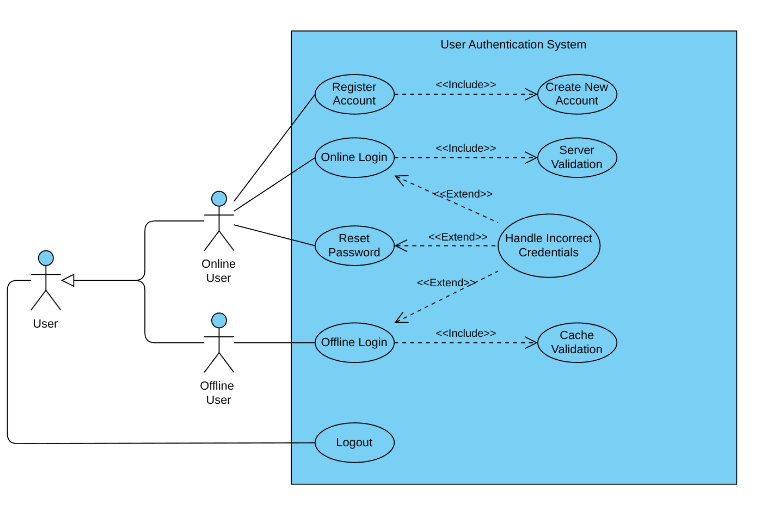
\includegraphics[width=0.9\textwidth]{registration_login.png}
  \caption{Registration and Login Use Case Diagram}
  \label{fig:reg-log-use-case}
\end{figure}

\subsection{Accessibility and Customization Use Case Diagram}
\begin{figure}[H]
  \centering
  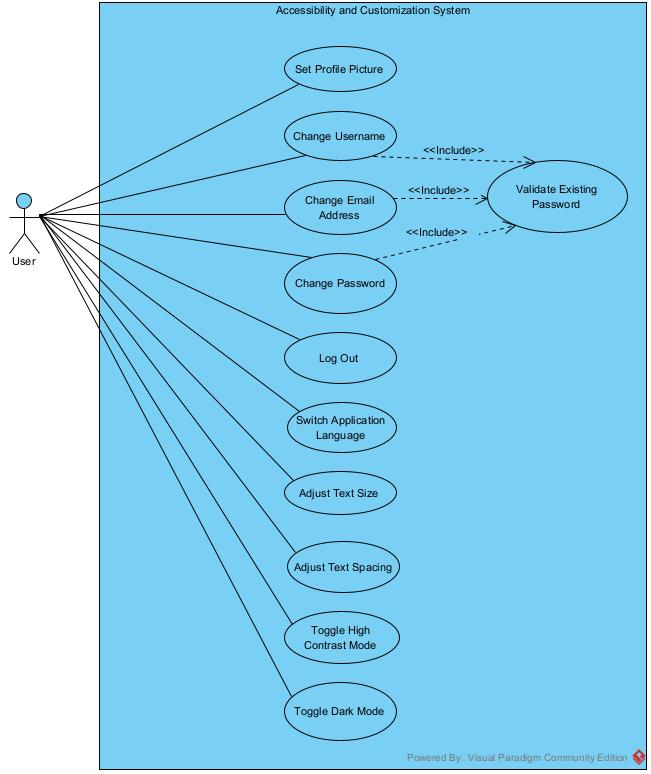
\includegraphics[width=0.9\textwidth]{Accessibility and Customization System.jpg}
  \caption{Accessibility and Customization Use Case Diagram for Marito}
  \label{fig:accessibility-customization-use-case}
\end{figure}

\subsection{Search Term Use Case Diagram}
\begin{figure}[H]
  \centering
  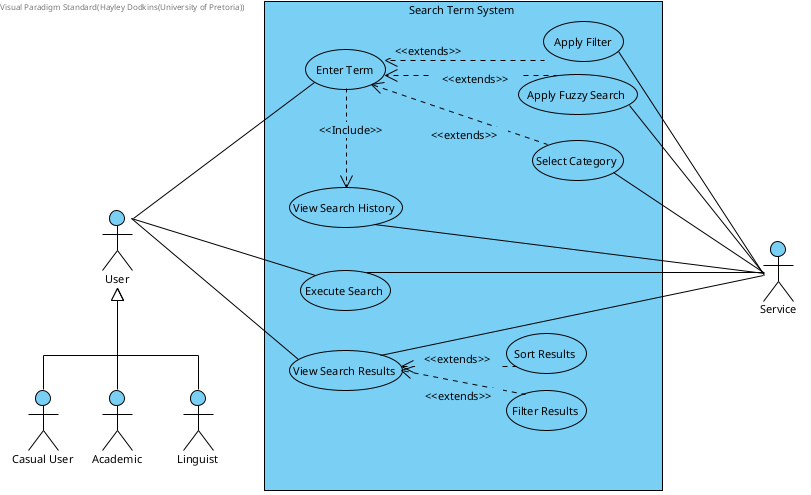
\includegraphics[width=0.9\textwidth]{SearchTermUseCase.png}
  \caption{Search Term Use Case Diagram for Marito}
  \label{fig:search-use-case}
\end{figure}

\subsection{Gamification Use Case Diagram}
\begin{figure}[H]
  \centering
  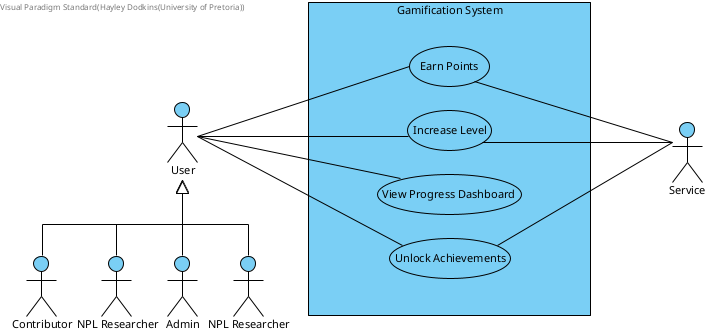
\includegraphics[width=0.9\textwidth]{GamifictionUseCase.png}
  \caption{Gamification Use Case Diagram}
  \label{fig:gamification-use-case}
\end{figure}

\subsection{Visualization Use Case Diagram}
\begin{figure}[H]
  \centering
  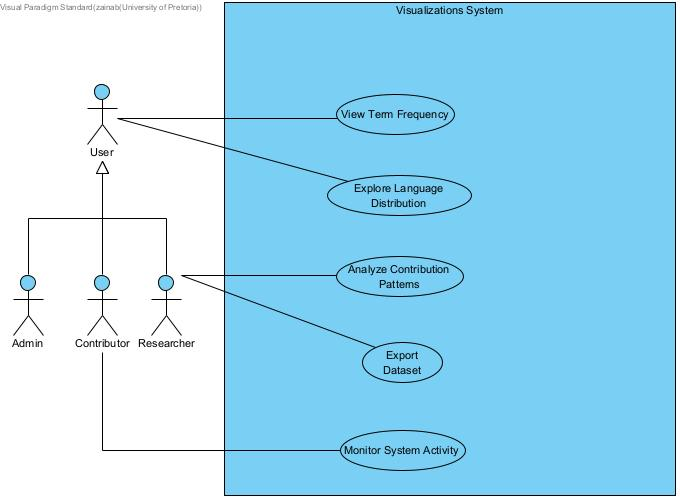
\includegraphics[width=0.9\textwidth]{Visualizations.jpg}
  \caption{Visualization Use Case Diagram}
  \label{fig:visualization-use-case}
\end{figure}

\subsection{Contributions Use Case Diagram}
\begin{figure}[H]
  \centering
  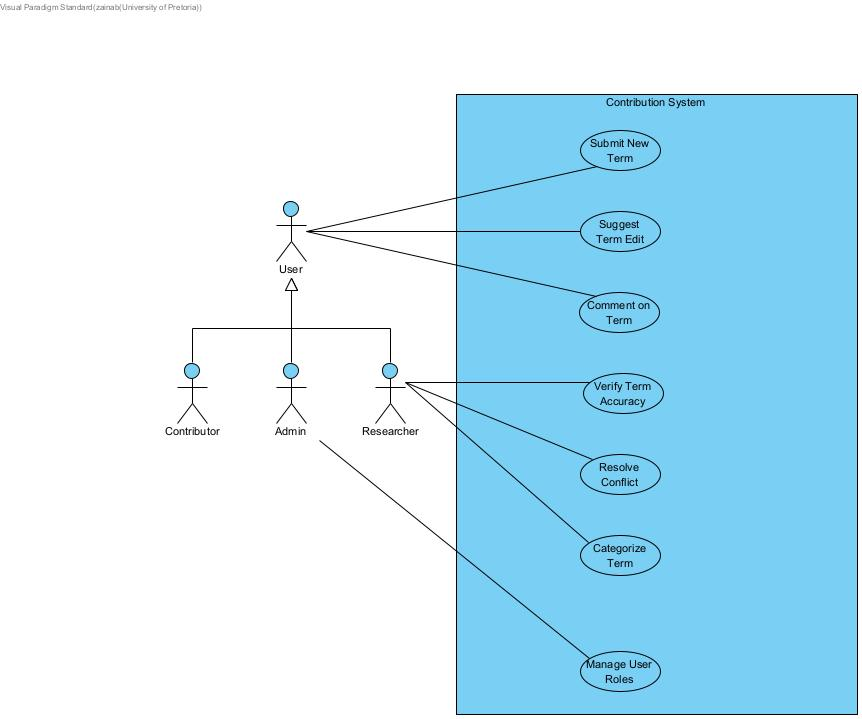
\includegraphics[width=0.9\textwidth]{Contributions.jpg}
  \caption{Contributions Use Case Diagram}
  \label{fig:contributions-use-case}
\end{figure}

\subsection{Dictionary Use Case Diagram}
\begin{figure}[H]
  \centering
  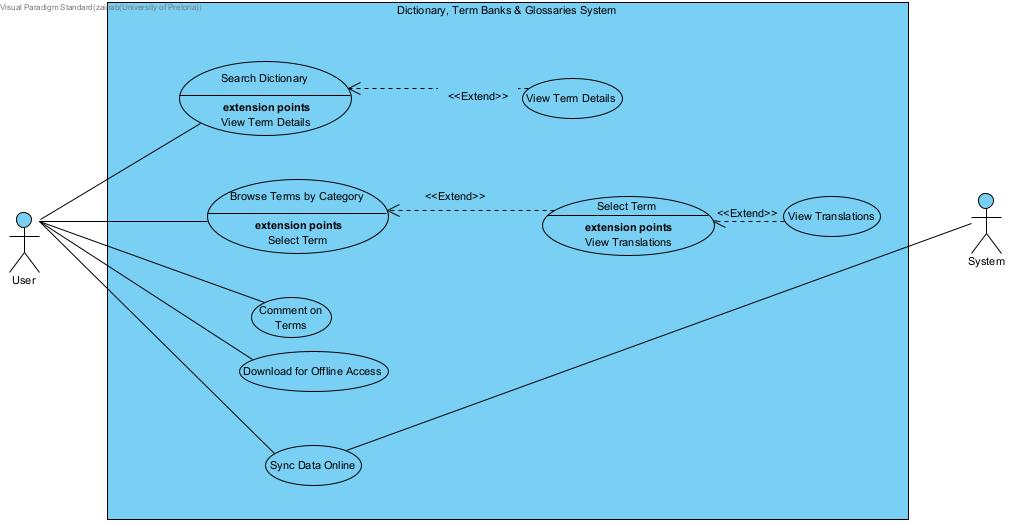
\includegraphics[width=0.9\textwidth]{Dictionary,Glossaies and Term Banl.jpg}
  \caption{Dictionary and Glossary Use Case Diagram}
  \label{fig:dictionary-use-case}
\end{figure}

\subsection{Admin Use Case Diagram}
\begin{figure}[H]
  \centering
  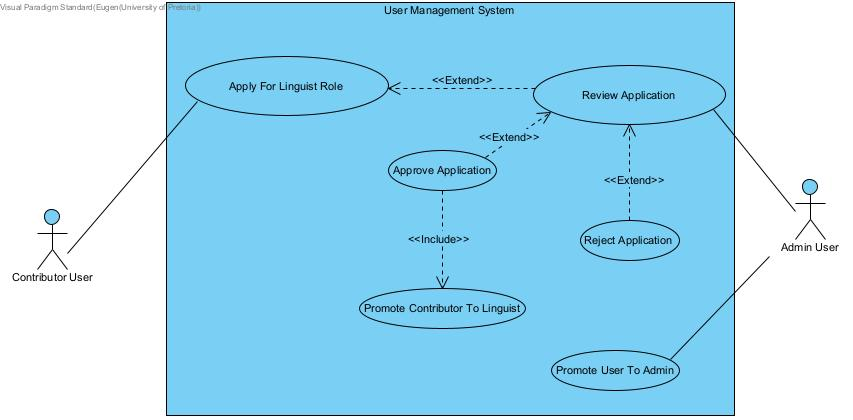
\includegraphics[width=0.9\textwidth]{Admin-User-Management.jpg}
  \caption{Admin User Management Use Case Diagram}
  \label{fig:admin-use-case}
\end{figure}

\subsection{Export Use Case Diagram}
\begin{figure}[H]
  \centering
  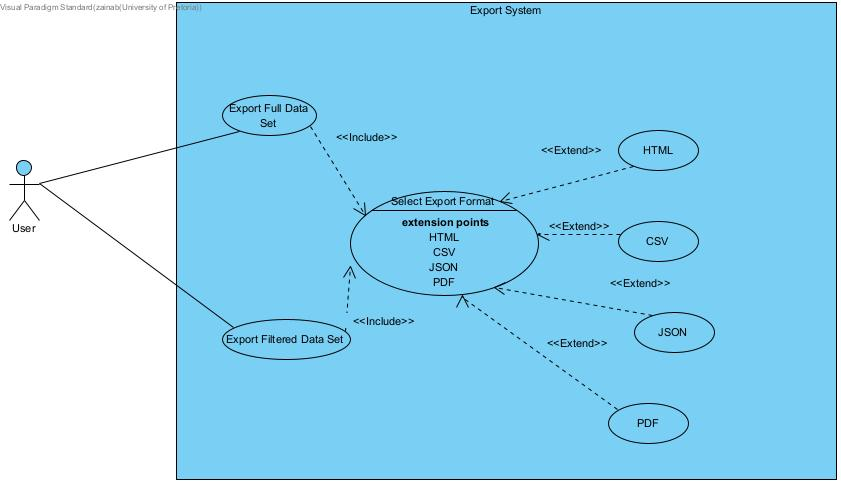
\includegraphics[width=0.9\textwidth]{Export System.jpg}
  \caption{Export System Use Case Diagram}
  \label{fig:export-use-case}
\end{figure}

\subsection{Feedback System Use Case Diagram}
\begin{figure}[H]
  \centering
  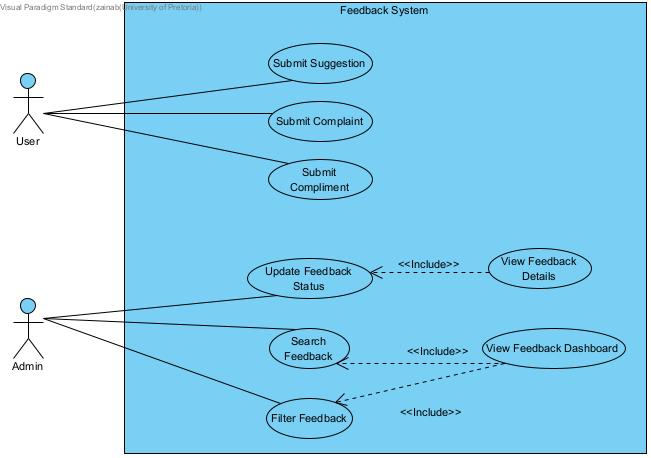
\includegraphics[width=0.9\textwidth]{Feedaback system.jpg}
  \caption{Feedback System Use Case Diagram}
  \label{fig:feedback-system-use-case}
\end{figure}

\subsection{Workspace Use Case Diagram}
\begin{figure}[H]
  \centering
  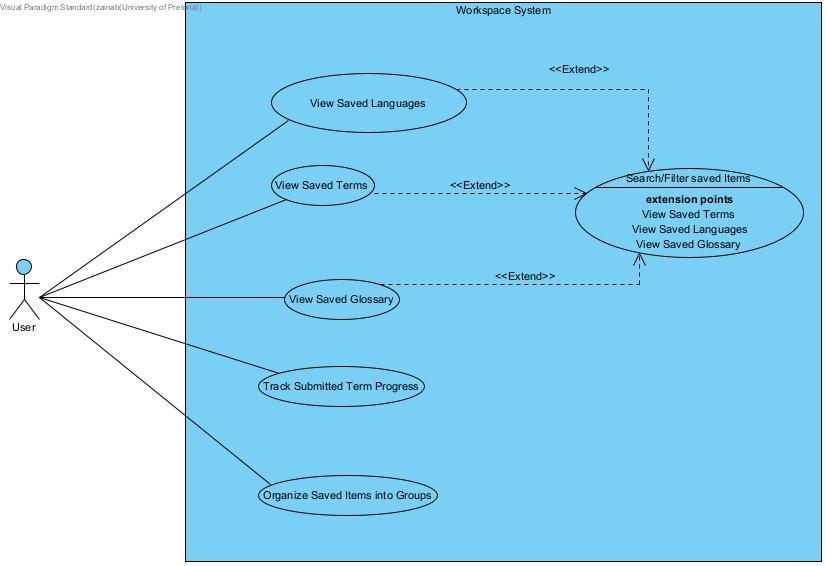
\includegraphics[width=0.9\textwidth]{workspace.jpg}
  \caption{Workspace Management Use Case Diagram}
  \label{fig:workspace-use-case}
\end{figure}

\subsection{Overview}
The main use cases covered include:
\begin{itemize}
  \item Browsing and searching multilingual terms
  \item Accessibility and customization
  \item Earning contribution points through gamified interactions
  \item Registration and login interactions
  \item User Contributions
  \item Data visualizations
  \item Dictionary Use Case
  \item Admin Use case
  \item Export Use Case
  \item Feedback System Use Case
  \item Workspace Management Use Case
\end{itemize}

\section{Functional Requirements}

\begin{enumerate}[label=FR\arabic*:, leftmargin=2.5em]

    \item \textbf{Glossary Browsing and Search}
    \begin{itemize}
        \item FR1.1: The system shall allow users to browse available glossaries and term banks.
        \item FR1.2: The system shall provide a unified search interface across all multilingual glossaries.
        \item FR1.3: The system shall allow users to search for terms using exact matches, partial strings, or semantic similarity.
        \item FR1.4: The search results shall be ranked by relevance and display key metadata (definition, part of speech, language).
        \item FR1.5: The system shall highlight related terms and translations in the term view.
    \end{itemize}

    \item \textbf{Accessibility and Customization}
    \begin{itemize}
        \item FR2.1: Profile \& Account Management
        \begin{itemize}
            \item FR2.1.1: The system shall allow users to upload and change profile pictures.
            \item FR2.1.2: The system shall enable username updates with real-time validation for uniqueness.
            \item FR2.1.3: The system shall require password validation before email changes and send verification emails.
            \item FR2.1.4: The system shall enforce secure password changes requiring current password validation.
            \item FR2.1.5: The system shall provide secure logout that terminates all sessions.
        \end{itemize}
        
        \item FR2.2: Multilingual Support
        \begin{itemize}
            \item FR2.2.1: The system shall support interface localization in all eleven official South African languages including English, Afrikaans, isiZulu, isiXhosa, Sesotho, Setswana, Sepedi, isiSwati, Tshivenda, Xitsonga, and isiNdebele.
            \item FR2.2.2: The system shall allow users to switch UI language anytime through settings.
            \item FR2.2.3: The system shall correctly render special characters for all supported languages.
            \item FR2.2.4: The system shall persist language preferences across sessions.
            \item FR2.2.5: The system shall apply language changes immediately without page refresh.
        \end{itemize}
        
        \item FR2.3: Text \& Visual Presentation
        \begin{itemize}
            \item FR2.3.1: The system shall allow users to adjust text size and display current size in pixels (e.g., 16px).
            \item FR2.3.2: The system shall provide real-time text size adjustment.
            \item FR2.3.3: The system shall show current text size value as users make changes.
            \item FR2.3.4: The system shall maintain text size preferences across sessions.
            \item FR2.3.5: The system shall ensure text scaling maintains proper layout.
        \end{itemize}
        
        \item FR2.4: Text Spacing Control
        \begin{itemize}
            \item FR2.4.1: The system shall allow users to adjust text spacing and display current multiplier (e.g., 1x).
            \item FR2.4.2: The system shall provide real-time spacing adjustment.
            \item FR2.4.3: The system shall show current spacing value as users make changes.
            \item FR2.4.4: The system shall apply spacing changes to all text elements consistently.
            \item FR2.4.5: The system shall preserve spacing preferences across sessions.
        \end{itemize}
        
        \item FR2.5: Colour \& Contrast Controls
        \begin{itemize}
            \item FR2.5.1: The system shall allow users to enable/disable High Contrast Mode.
            \item FR2.5.2: The system shall show current mode state (on/off).
            \item FR2.5.3: The system shall increase color contrast when high contrast mode is enabled.
            \item FR2.5.4: The system shall maintain high contrast settings across sessions.
            \item FR2.5.5: The system shall ensure interactive elements remain distinguishable in high contrast mode.
        \end{itemize}
        
        \item FR2.6: Dark Mode
        \begin{itemize}
            \item FR2.6.1: The system shall allow users to enable/disable Dark Mode.
            \item FR2.6.2: The system shall show current mode state (on/off).
            \item FR2.6.3: The system shall apply dark backgrounds with light text when enabled.
            \item FR2.6.4: The system shall maintain proper contrast in dark mode.
            \item FR2.6.5: The system shall preserve dark mode preferences across sessions.
            \item FR2.6.6: The system shall provide smooth transitions when switching modes.
        \end{itemize}
    \end{itemize}

    \item \textbf{User Contributions and Feedback}
    \begin{itemize}
        \item FR3.1: The system shall allow users to submit comments.
        \item FR3.2: The system shall allow users to submit corrections or suggestions for terms.
        \item FR3.3: The system shall send submitted feedback to a backend repository for moderation.
        \item FR3.4: The system shall support version control for submitted glossary data and prevent overwriting of validated entries.
        \item FR3.5: The system should be able to allow users to upvote/downvote term changes.
    \end{itemize}

    \item \textbf{AI-Enhanced Functionality}
    \begin{itemize}
        \item FR4.1: The system shall support AI-powered semantic search to retrieve conceptually related terms.
        \item FR4.2: The system may provide suggested definitions or translations using AI models.
        \item FR4.3: The system may automatically cluster terms based on meaning or domain.
        \item FR4.4: The system may auto-tag glossary entries with linguistic metadata (e.g., part-of-speech).
        \item FR4.5: The system may integrate with external NLP APIs for research purposes.
    \end{itemize}

    \item \textbf{Gamification}
    \begin{itemize}
        \item FR5.1: The system shall assign points to users when they submit valid suggestions, comments, or issue reports on glossary terms.
        \item FR5.2: The system shall track milestones based on user activity and unlock achievements or badges when predefined thresholds are reached.
        \item FR5.3: The system shall display a progress dashboard on the user's profile page, including total points, badges earned, and contribution rank.
        \item FR5.4: The system shall provide real-time feedback when users perform actions that affect their gamification status.
        \item FR5.5: The system shall support user rank or title progression as users accumulate points and reach specific contribution levels.
        \item FR5.6: The system shall queue gamified contributions made offline and synchronize them with the server once the user is reconnected.
        \item FR5.7: The system shall validate contributions before assigning gamification points to prevent abuse.
    \end{itemize}

    \item \textbf{Progressive Web Application Functionality}
    \begin{itemize}
        \item FR6.1: The system shall function as a PWA and be installable on mobile and desktop devices.
        \item FR6.2: The frontend shall use service workers to cache glossary data, enabling offline access to core features such as term lookup and browsing.
        \item FR6.3: The system shall store user feedback or contributions made offline and queue them for submission once connectivity is restored.
        \item FR6.4: The application shall automatically synchronize cached content with the server when an internet connection is detected.
        \item FR6.5: The system shall provide visual feedback or indicators when the app is operating in offline mode.
        \item FR6.6: The system shall support background updates of cached glossary data to maintain consistency with the server.
        \item FR6.8: The system shall allow users to download selected glossaries for offline access.
    \end{itemize}

    \item \textbf{Data Visualization and Analytics}
    \begin{itemize}
        \item FR7.1: The system should be able to display stats on word frequency and usage trends.
        \item FR7.2: The system should be able to visualize a user's contribution to different languages.
        \item FR7.3: The system should highlight trending words and new entries to the database.
        \item FR7.4: The system should be able to provide interactive charts or graphs for linguistic data.
    \end{itemize}

    \item \textbf{Data Import and Export}
    \begin{itemize}
        \item FR8.1: The system shall allow users to export glossary data in JSON format.
        \item FR8.2: The system shall allow users to export glossary data in CSV format.
        \item FR8.3: The system may allow authorized users to import glossaries in JSON or CSV format.
    \end{itemize}

    \item \textbf{Feedback System}
    \begin{itemize}
        \item FR9.1: \textbf{Feedback Submission}
        \begin{itemize}
            \item FR9.1.1: The system shall allow users to submit feedback through multiple categories: Suggestion, Complaint, and Compliment.
            \item FR9.1.2: The system shall allow users to optionally provide their name and email address with feedback submissions.
            \item FR9.1.3: The system shall require a descriptive message for all feedback submissions.
            \item FR9.1.4: The system shall validate that required fields are completed before allowing submission.
            \item FR9.1.5: The system shall provide appropriate guidance text based on the selected feedback category.
            \item FR9.1.6: The system shall accept anonymous feedback submissions when contact information is not provided.
        \end{itemize}
        \item FR9.2: \textbf{Feedback Administration}
        \begin{itemize}
            \item FR9.2.1: The system shall provide administrators with a dashboard showing feedback statistics and trends.
            \item FR9.2.2: The system shall display all feedback items with category, status, priority, user information, and submission date.
            \item FR9.2.3: The system shall allow administrators to filter feedback by type (suggestions, complaints, compliments) and status (pending, in-progress, resolved).
            \item FR9.2.4: The system shall provide search functionality across feedback content and user information.
            \item FR9.2.5: The system shall allow administrators to update the status of feedback items through a defined workflow.
            \item FR9.2.6: The system shall track all status changes with timestamps for audit purposes.
        \end{itemize}
    \end{itemize}

    \item \textbf{Workspace Management}
    \begin{itemize}
        \item FR10.1: The system shall provide a personalized workspace where users can organize, access, and manage their saved language resources and contributions.
        \item FR10.2: \textbf{Saved Terms}
        \begin{itemize}
            \item FR10.2.1: The system shall allow users to bookmark individual terms from dictionaries/glossaries for quick access.
            \item FR10.2.2: The system shall display saved terms in a searchable, filterable list (e.g., by language, tags, or date saved).
            \item FR10.2.3: The system shall enable users to add custom notes or annotations to saved terms.
            \item FR10.2.4: The system shall sync saved terms across devices when online and when offline.
        \end{itemize}
        \item FR10.3: \textbf{Saved Glossaries}
        \begin{itemize}
            \item FR10.3.1: The system shall allow users to download entire glossaries/dictionaries for offline access.
            \item FR10.3.2: The system shall let users mark glossaries as "favorites" for quick filtering.
            \item FR10.3.3: The system shall notify users when a saved glossary has updates (e.g., new terms or corrections).
            \item FR10.3.4: The system shall provide storage management (e.g., "Delete Glossary" to free space).
        \end{itemize}
        \item FR10.4: \textbf{Contributed Terms}
        \begin{itemize}
            \item FR10.4.1: The system shall maintain a history of user-submitted terms, definitions, or edits.
            \item FR10.4.2: The system shall display the moderation status of contributions (e.g., "Pending," "Approved," "Rejected").
        \end{itemize}
        \item FR10.5: \textbf{Workspace Organization}
        \begin{itemize}
            \item FR10.5.1: The system shall allow users to create folders/tags to group saved terms or glossaries (e.g., "Thesis Research").
            \item FR10.5.2: The system shall support bulk actions (e.g., "Move 5 terms to Folder X").
        \end{itemize}
    \end{itemize}

\end{enumerate}


\section{Non-Functional Requirements}

\begin{enumerate}[label=NFR\arabic*:, leftmargin=2.5em]
    \item \textbf{Offline Accessibility}
    \begin{itemize}
        \item NFR1.1 The system shall support offline access to previously downloaded language resources.
        \item NFR1.2 The frontend shall use service workers and caching to allow uninterrupted use of core features without an active internet connection.
        \item NFR1.3 Synchronization of updated resources shall automatically occur once the device is back online.
    \end{itemize}
    
    \item \textbf{Performance and Responsiveness}
    \begin{itemize}
        \item NFR2.1 The system shall deliver fast search responses, with results displayed within 2 seconds for standard queries.
        \item NFR2.2 The frontend application shall load and become interactive within 3 seconds on devices with moderate hardware and average bandwidth.
        \item NFR2.3 UI interactions shall be smooth and not exceed 100ms latency where possible.
    \end{itemize}
    
    \item \textbf{Scalability}
    \begin{itemize}
        \item NFR3.1 The backend shall be able to handle simultaneous requests from a growing user base, including researchers and contributors.
        \item NFR3.2 The data architecture must accommodate the addition of new glossaries, languages, and APIs without the need for major refactoring.
    \end{itemize}
    
    \item \textbf{Security and Privacy}
    \begin{itemize}
        \item NFR4.1 All data transmissions between client and server shall be encrypted using HTTPS.
        \item NFR4.2 User-submitted feedback shall be sanitized and validated to prevent injection attacks.
        \item NFR4.3 The backend shall implement basic access control to restrict sensitive actions to authorized roles.
    \end{itemize}
    
    \item \textbf{Usability and Accessibility}
    \begin{itemize}
        \item NFR5.1 The user interface shall support all 11 official South African languages through dynamic localization.
        \item NFR5.2 The application shall conform to WCAG 2.1 Level AA accessibility guidelines to accommodate visually impaired users.
        \item NFR5.3 The system shall provide a clean and intuitive interface that requires no more than three clicks to reach key features.
    \end{itemize}
    
    \item \textbf{Maintainability}
    \begin{itemize}
        \item NFR6.1 The codebase shall follow modular and well-documented design practices to enable ease of maintenance.
        \item NFR6.2 The frontend and backend shall use consistent code formatting enforced via linting tools.
        \item NFR6.3 New contributors shall be able to understand and modify the codebase with minimal onboarding effort.
    \end{itemize}
    
    \item \textbf{Extensibility}
    \begin{itemize}
        \item NFR7.1 The system shall support the addition of new term banks and glossaries via a modular import system.
        \item NFR7.2 New frontend features shall be integrable without affecting the core application features.
        \item NFR7.3 The backend shall expose extensible REST API routes following OpenAPI standards.
    \end{itemize}
    
    \item \textbf{Reliability and Fault Tolerance}
    \begin{itemize}
        \item NFR8.1 The system shall gracefully handle failed API requests and notify the user when a feature is temporarily unavailable.
        \item NFR8.2 The frontend shall include fallback mechanisms for critical resources, ensuring minimal disruption in case of partial data loss.
        \item NFR8.3 The backend shall log all failed operations and expose logs for future debugging or auditing.
    \end{itemize}
    
    \item \textbf{Portability and Cross-Platform Compatibility}
    \begin{itemize}
        \item NFR9.1 The PWA shall work on major browsers (Chrome, Firefox, Edge, Safari) and platforms (Windows, Android, iOS, Linux).
        \item NFR9.2 The UI shall be fully responsive and usable on screen sizes ranging from smartphones to desktop monitors.
        \item NFR9.3 No feature shall be dependent on platform-specific behavior.
    \end{itemize}
    
    \item \textbf{Deployment and DevOps Readiness}
    \begin{itemize}
        \item NFR10.1 The backend shall be containerized using Docker to support consistent deployment across environments.
        \item NFR10.2 CI/CD pipelines shall be configured to run tests, build artifacts, and deploy the application to the cloud or GitHub Pages.
    \end{itemize}
\end{enumerate}


\section{Constraints}

\subsection{Overview}
This section outlines the constraints that govern the design, development, deployment, and maintenance of the \textbf{Marito} application. These constraints stem from ethical considerations, client requirements, project context, budgetary limitations, and architectural guidelines. Adherence to these constraints is critical to the project's success and sustainability.

\subsection{Constraints}

\begin{enumerate}[label=2.\arabic*, leftmargin=2.5em]

    \item \textbf{Privacy and Data Minimization}
    \begin{itemize}
        \item The application must adopt a privacy-first approach.
        \item No personal user information may be collected unless voluntarily submitted.
        \item No personal data should be stored without explicit user consent.
        \item Any user data collected must comply with ethical research standards and university data policies.
        \item All stored data must follow ethical and data protection principles.
    \end{itemize}

    \item \textbf{Maintainability and Sustainability}
    \begin{itemize}
        \item The project must use a maintainable and reliable technology stack that future students or stakeholders can easily understand and extend.
        \item All source code must be well-documented, modular, and follow clean architecture principles.
        \item Technologies selected must have active community support and comprehensive documentation to minimize onboarding effort.
    \end{itemize}

    \item \textbf{Use of Open Source Technologies}
    \begin{itemize}
        \item Wherever possible, the project must use open-source frameworks and libraries.
        \item External packages or modules must have permissive licenses (e.g., MIT, Apache 2.0) and be cited appropriately.
    \end{itemize}

    \item \textbf{Budget Constraints}
    \begin{itemize}
        \item The project must be developed with minimal to zero cost.
        \item The team is not permitted to incur costs unless explicitly approved by the client.
        \item Hosting should utilize free tiers.
    \end{itemize}

    \item \textbf{Offline Functionality}
    \begin{itemize}
        \item The application must support offline access as a core feature.
        \item Core features must function without an active internet connection, using Progressive Web App (PWA) technologies such as service workers and local caching.
        \item Synchronization with the central repository must occur seamlessly once connectivity is restored.
    \end{itemize}

    \item \textbf{Version Control of Glossary Data}
    \begin{itemize}
        \item Glossary data and language resources must be version-controlled to prevent loss or corruption of validated content.
        \item User feedback must be stored separately and reviewed before merging into the main dataset.
        \item No glossary data may be overwritten without proper validation and versioning mechanisms.
    \end{itemize}

    \item \textbf{Ethical and Legal Considerations}
    \begin{itemize}
        \item No proprietary or restricted datasets may be used without explicit authorization.
        \item Contributions and authorship must be tracked where possible to preserve academic and community recognition.
    \end{itemize}

    \item \textbf{Performance and Efficiency}
    \begin{itemize}
        \item The application must be responsive and performant on low-resource or mobile devices.
        \item Heavy assets (e.g., large datasets or images) must be lazy-loaded or paginated.
        \item Search and filtering mechanisms must be optimized for performance on slower devices and large datasets.
    \end{itemize}

    \item \textbf{Accessibility Requirements}
    \begin{itemize}
        \item The application must adhere to WCAG 2.1 AA accessibility standards.
        \item Features such as text-to-speech, keyboard navigation, color contrast, and screen reader support should be considered where feasible.
        \item Dark mode and adjustable text size are encouraged to support visual diversity in users.
    \end{itemize}

    \item \textbf{Deployment and Portability}
    \begin{itemize}
        \item The system must be deployable using containerization to support ease of testing and reproducibility.
        \item CI/CD pipelines must be used for automated builds and testing.
        \item Both frontend and backend should be deployable without manual intervention.
    \end{itemize}

    \item \textbf{Multi-Language Support}
    \begin{itemize}
        \item The interface must support multiple South African languages.
        \item The system must be internationalization-ready using industry-standard practices (e.g., translation JSON files, locale selectors).
        \item UI elements, glossaries, and feedback must render correctly regardless of language.
    \end{itemize}

\end{enumerate}

\subsection{Summary}
These constraints serve as the foundation for all architectural, design, and implementation decisions made during the development of \textbf{Marito}. They ensure the solution is ethical, sustainable, inclusive, affordable, and aligned with the client’s goals of making multilingual resources accessible to all.


\section{Domain Model}
\begin{figure}[H]
  \centering
  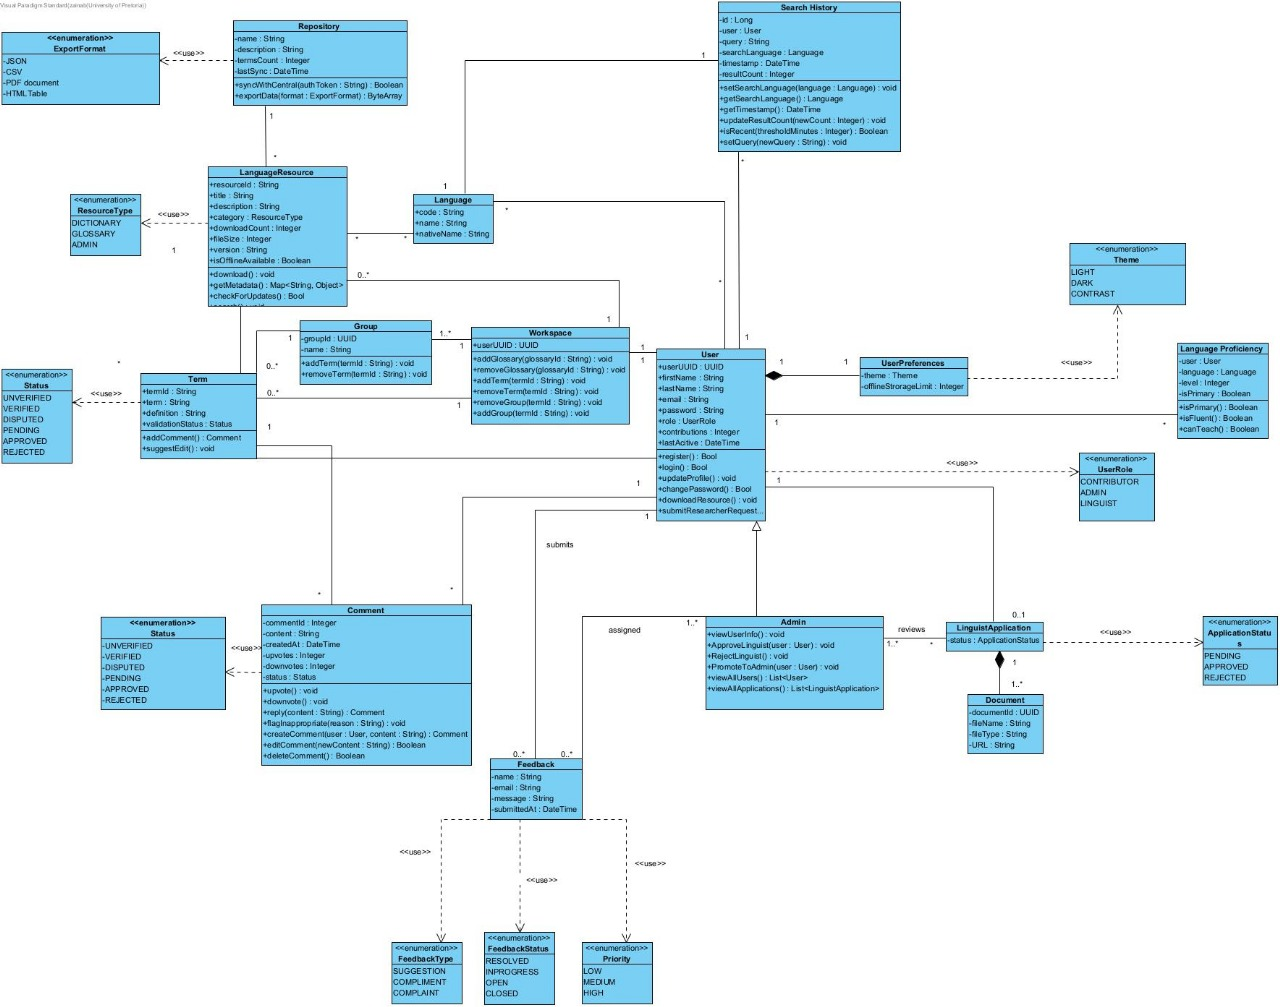
\includegraphics[width=0.9\textwidth]{domain_model_V1.1.0.jpg}
  \caption{Domain Model}
  \label{fig:domain-model}
\end{figure}

\href{https://github.com/COS301-SE-2025/Marito/blob/develop/Documentation/System%20Requirements/Architectural_Specifications_v4.pdf}{Architectural Specifications \& Service Contract}

\end{document}
